\section{Procedimientos.}

	\begin{itemize}
		\subsection{Parte 1. Iniciando Docker.}
			\item Abrimos nuestro menú de inicio y buscamos la aplicación Docker for Windows.
				\begin{figure}[htb]
					\begin{center}
						
\includegraphics[width=8cm]{./Imagenes/BuscarDocker}
					\end{center}
				\end{figure}
			\item Una vez iniciado se podrá visualizar el icono de Docker en el área de notificación.
				\begin{figure}[htb]
					\begin{center}
						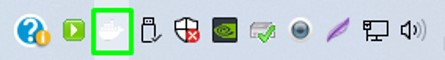
\includegraphics[width=6cm]{./Imagenes/VerIcono}
					\end{center}
				\end{figure}
			\item Asimismo se podrá visualizar la ventana de bienvenida.
				\begin{figure}[htb]
					\begin{center}
						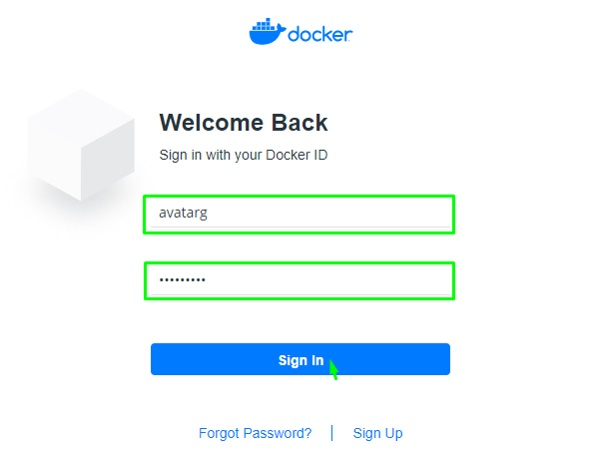
\includegraphics[width=9cm]{./Imagenes/Loguearse}
					\end{center}
				\end{figure}
			\item El resultado sería como se muestra en la siguiente imagen.
					\begin{figure}[htb]
						\begin{center}
							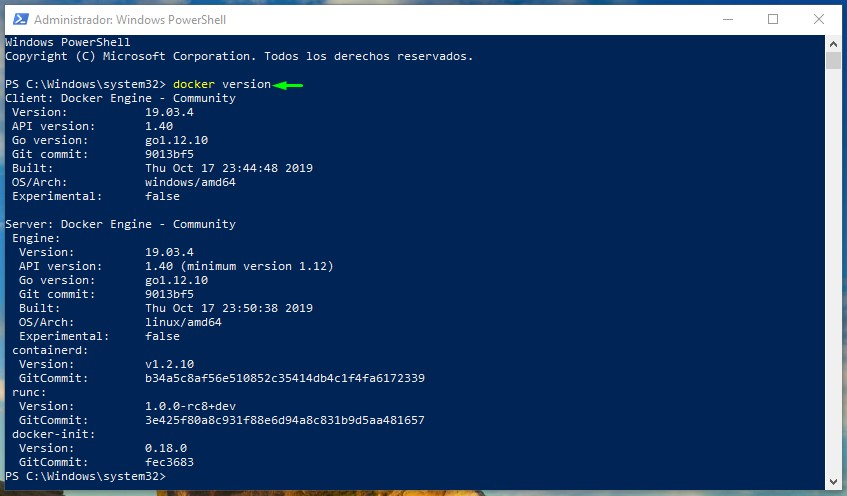
\includegraphics[width=16cm]{./Imagenes/VersionDocker}
						\end{center}
					\end{figure}
				\vspace{7cm}
		\subsection{Parte 2. Ceando un Contenedor son Oracle Database para Linux.}
			\item Ingresamos a Nuestro Buscador de Internet Google Chrome  o cualquier otro.
				\begin{figure}[htb]
					\begin{center}
						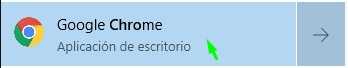
\includegraphics[width=8cm]{./Imagenes/BuscarAppGoogle}
					\end{center}
				\end{figure}
			\item Luego Copiamos y Pegamos el Siguiente Link.
				\begin{center}
					\url{https://hub.docker.com/}
				\end{center}
				\vspace{7cm}
			\item Inciamos Sesión o nos Creamos una Cuante Nueva.
				\begin{figure}[htb]
					\begin{center}
						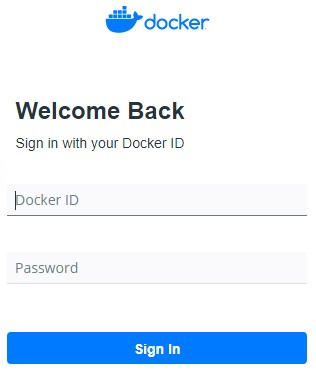
\includegraphics[width=6cm]{./Imagenes/Loguearse3}
					\end{center}
				\end{figure}				
			\item Seguidamente de loguearnos, seleccionamos la caja de texto de busqueda y digitamos lo siguiente:
				\begin{figure}[htb]
					\begin{center}
						
\includegraphics[width=9cm]{./Imagenes/BuscarOracleDatabase1}
					\end{center}
				\end{figure}
			\item Y seleccionamos la Primera Opción, tal y como se muestra en la siguiente imagen.
				\begin{figure}[htb]
					\begin{center}
						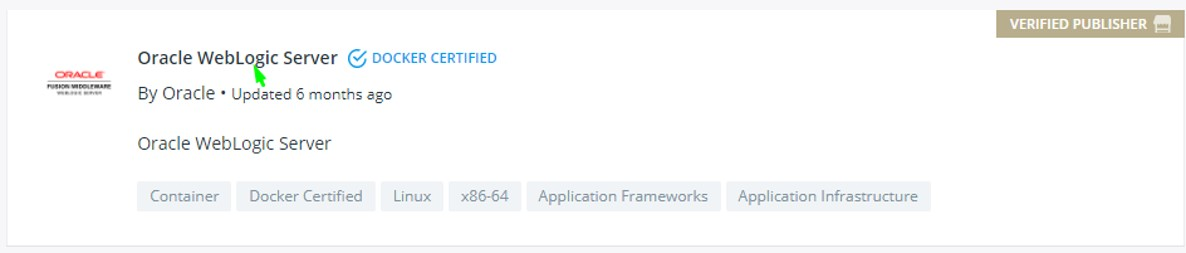
\includegraphics[width=15cm]{./Imagenes/Seleccionar1}
					\end{center}
				\end{figure}
			\item Procedemos con el CheckOut, seleccionando el boton indicado en la imagen.
				\begin{figure}[htb]
					\begin{center}
						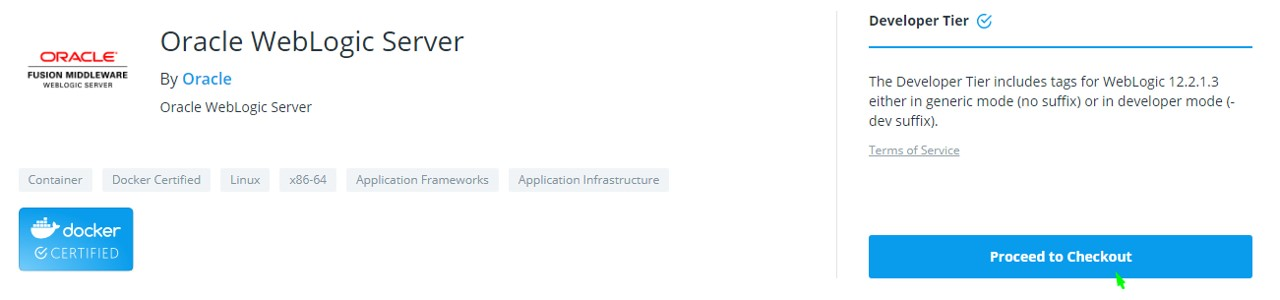
\includegraphics[width=15cm]{./Imagenes/Seleccionar2}
					\end{center}
				\end{figure}
				\vspace{5cm}
			\item Ingresamos las casillas y seleccionamos el boton indicado en la siguiente imagen.
				\begin{figure}[htb]
					\begin{center}
						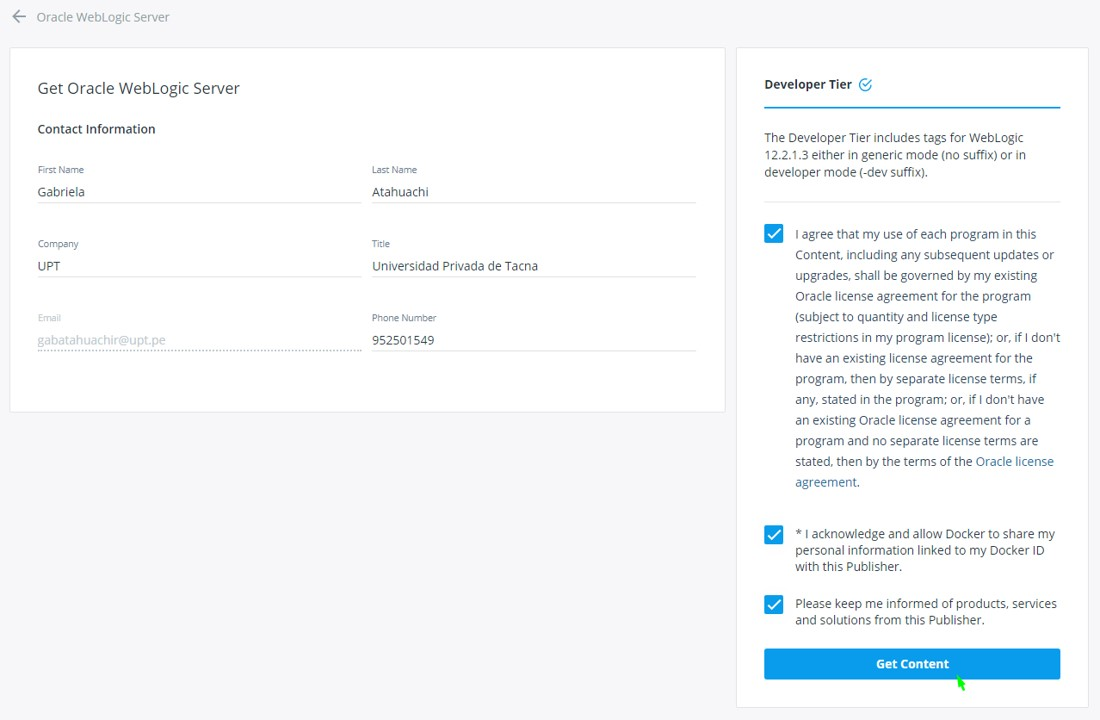
\includegraphics[width=15cm]{./Imagenes/Seleccionar3}
					\end{center}
				\end{figure}
			\item Al final obtenemos el acceso al contenido.
				\begin{figure}[htb]
					\begin{center}
						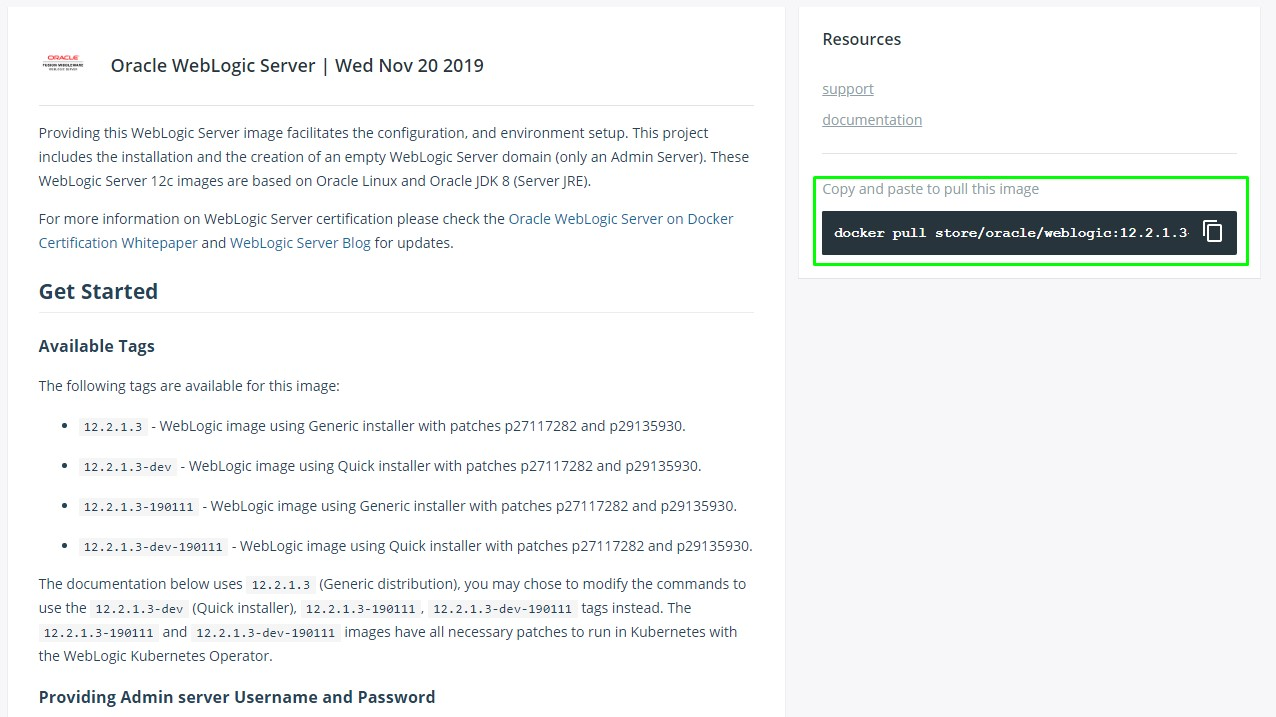
\includegraphics[width=15cm]{./Imagenes/Seleccionar4}
					\end{center}
				\end{figure}
				\vspace{7cm}
			\item Ahora buscamos el programa Windows PowerShell.
					\begin{figure}[htb]
						\begin{center}
							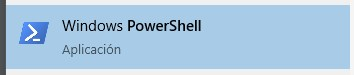
\includegraphics[width=8cm]{./Imagenes/BuscarPowerShell}
						\end{center}
					\end{figure}
				\item Luego lo ejecutamos como administrador para que no genere problemas luego.
					\begin{figure}[htb]
						\begin{center}
							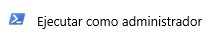
\includegraphics[width=6cm]{./Imagenes/EjecutarComoAdministrador}
						\end{center}
					\end{figure}
				\item Se mostrará una ventana como la que se ve en la imagen.
					\begin{figure}[htb]
						\begin{center}
							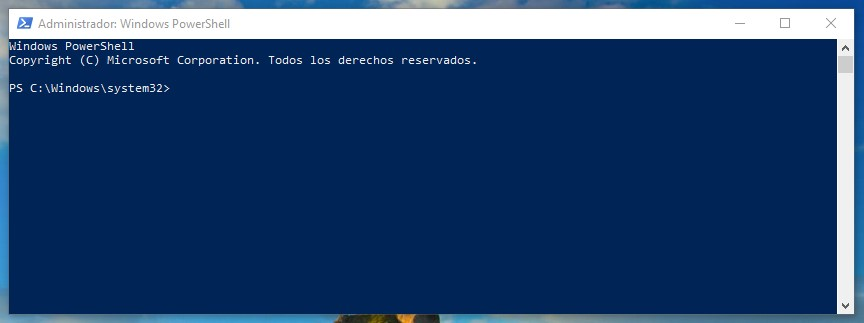
\includegraphics[width=16cm]{./Imagenes/InicioPowerShell}
						\end{center}
					\end{figure}
					\vspace{7cm}
				\item Digitaremos lo siguiente.
					\begin{figure}[htb]
						\begin{center}
							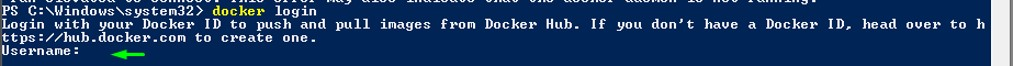
\includegraphics[width=16cm]{./Imagenes/Comando01}
						\end{center}
					\end{figure}
	\end{itemize}